\begin{figure*}
    \centering
    \vspace{-0.6cm}
    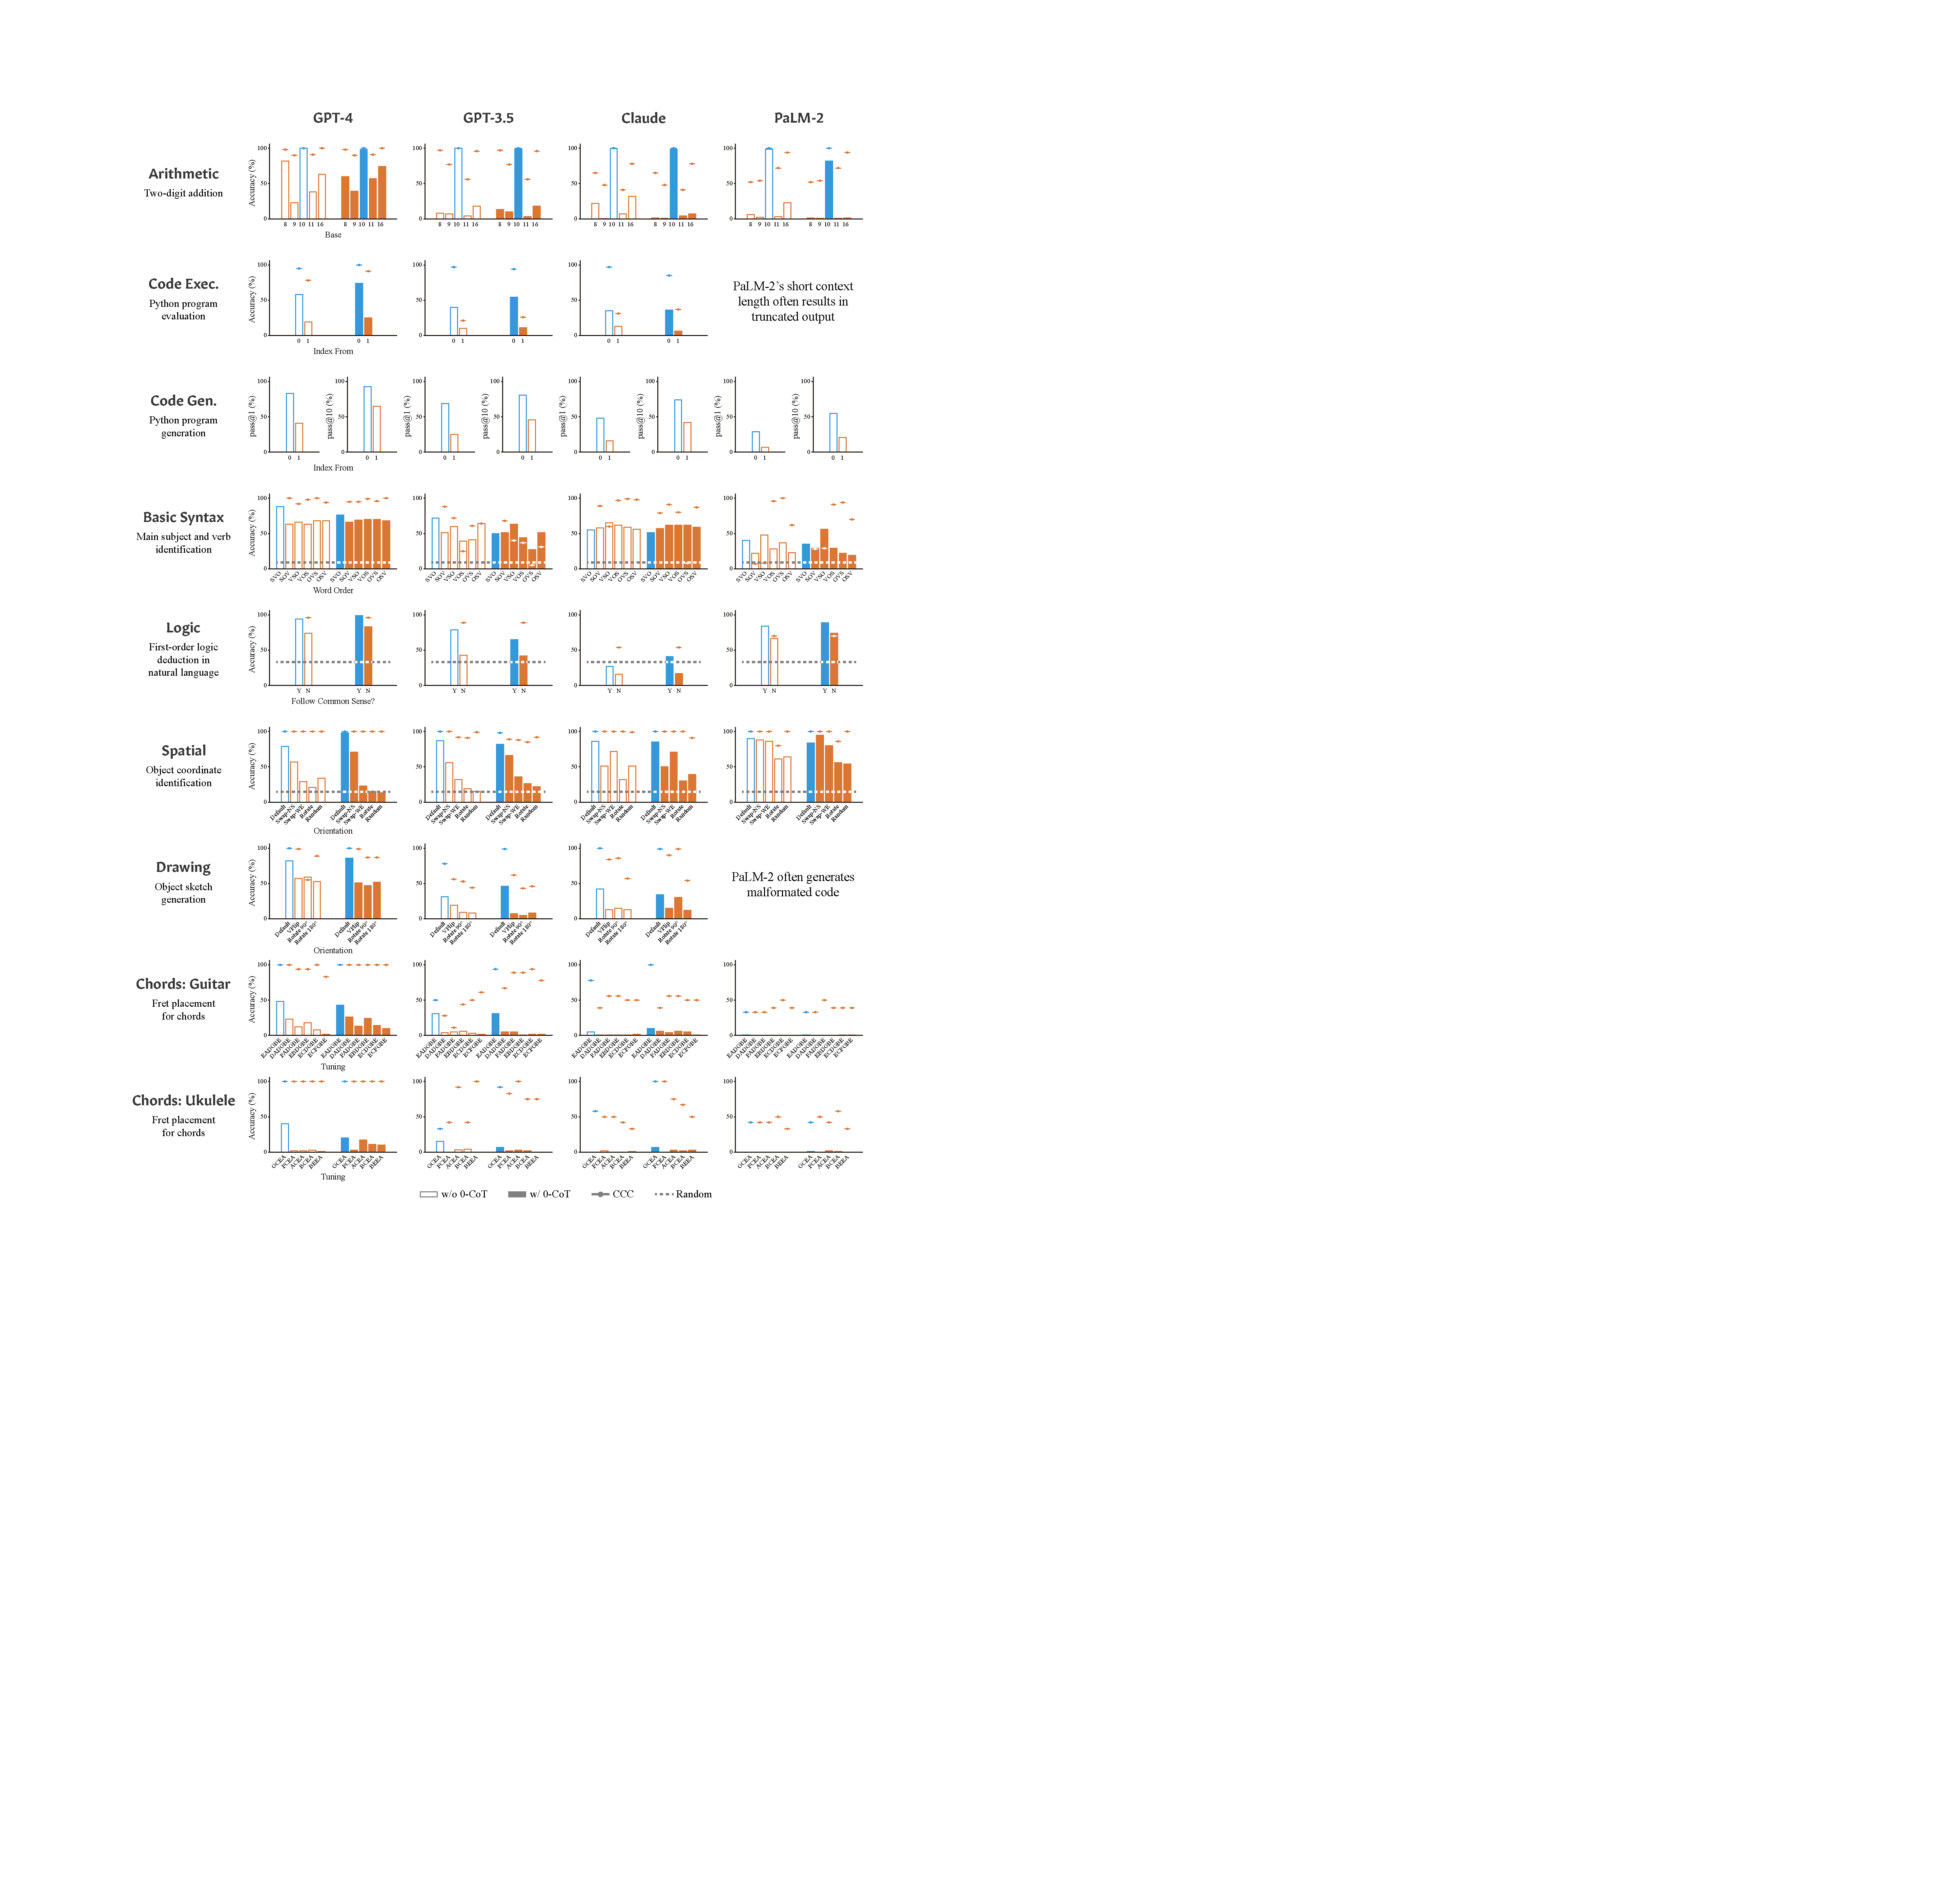
\includegraphics[width=\textwidth]{figures/results.pdf}
    \caption{
    Main results. The \textcolor{real}{blue} and \textcolor{cf}{orange} bars represent the \textcolor{real}{default} and \textcolor{cf}{counterfactual} conditions respectively, either  with or without 0-shot chain-of-thought (0-CoT) (except code generation; see \S\ref{sec:programming-setup}). CCC is the counterfactual comprehension check (\S\ref{subsec:ccc}), but when applicable, we report it for the default setting too.
    Random performance is marked whenever nontrivial.
    PaLM-2 here is not the largest version (\S\ref{sec:results}).
    The CCC for code execution/generation are identical. For spatial reasoning, we average the results from all rotation degrees.
    Counterfactual performance is consistently lower than the default task performance, while CCC is usually high.
    \S\ref{sec:raw-results} reports numeric results.}
    \vspace{-1cm}
    \label{fig:results-1}
\end{figure*}

\begin{figure*}
    \centering
    \vspace{-4mm}
    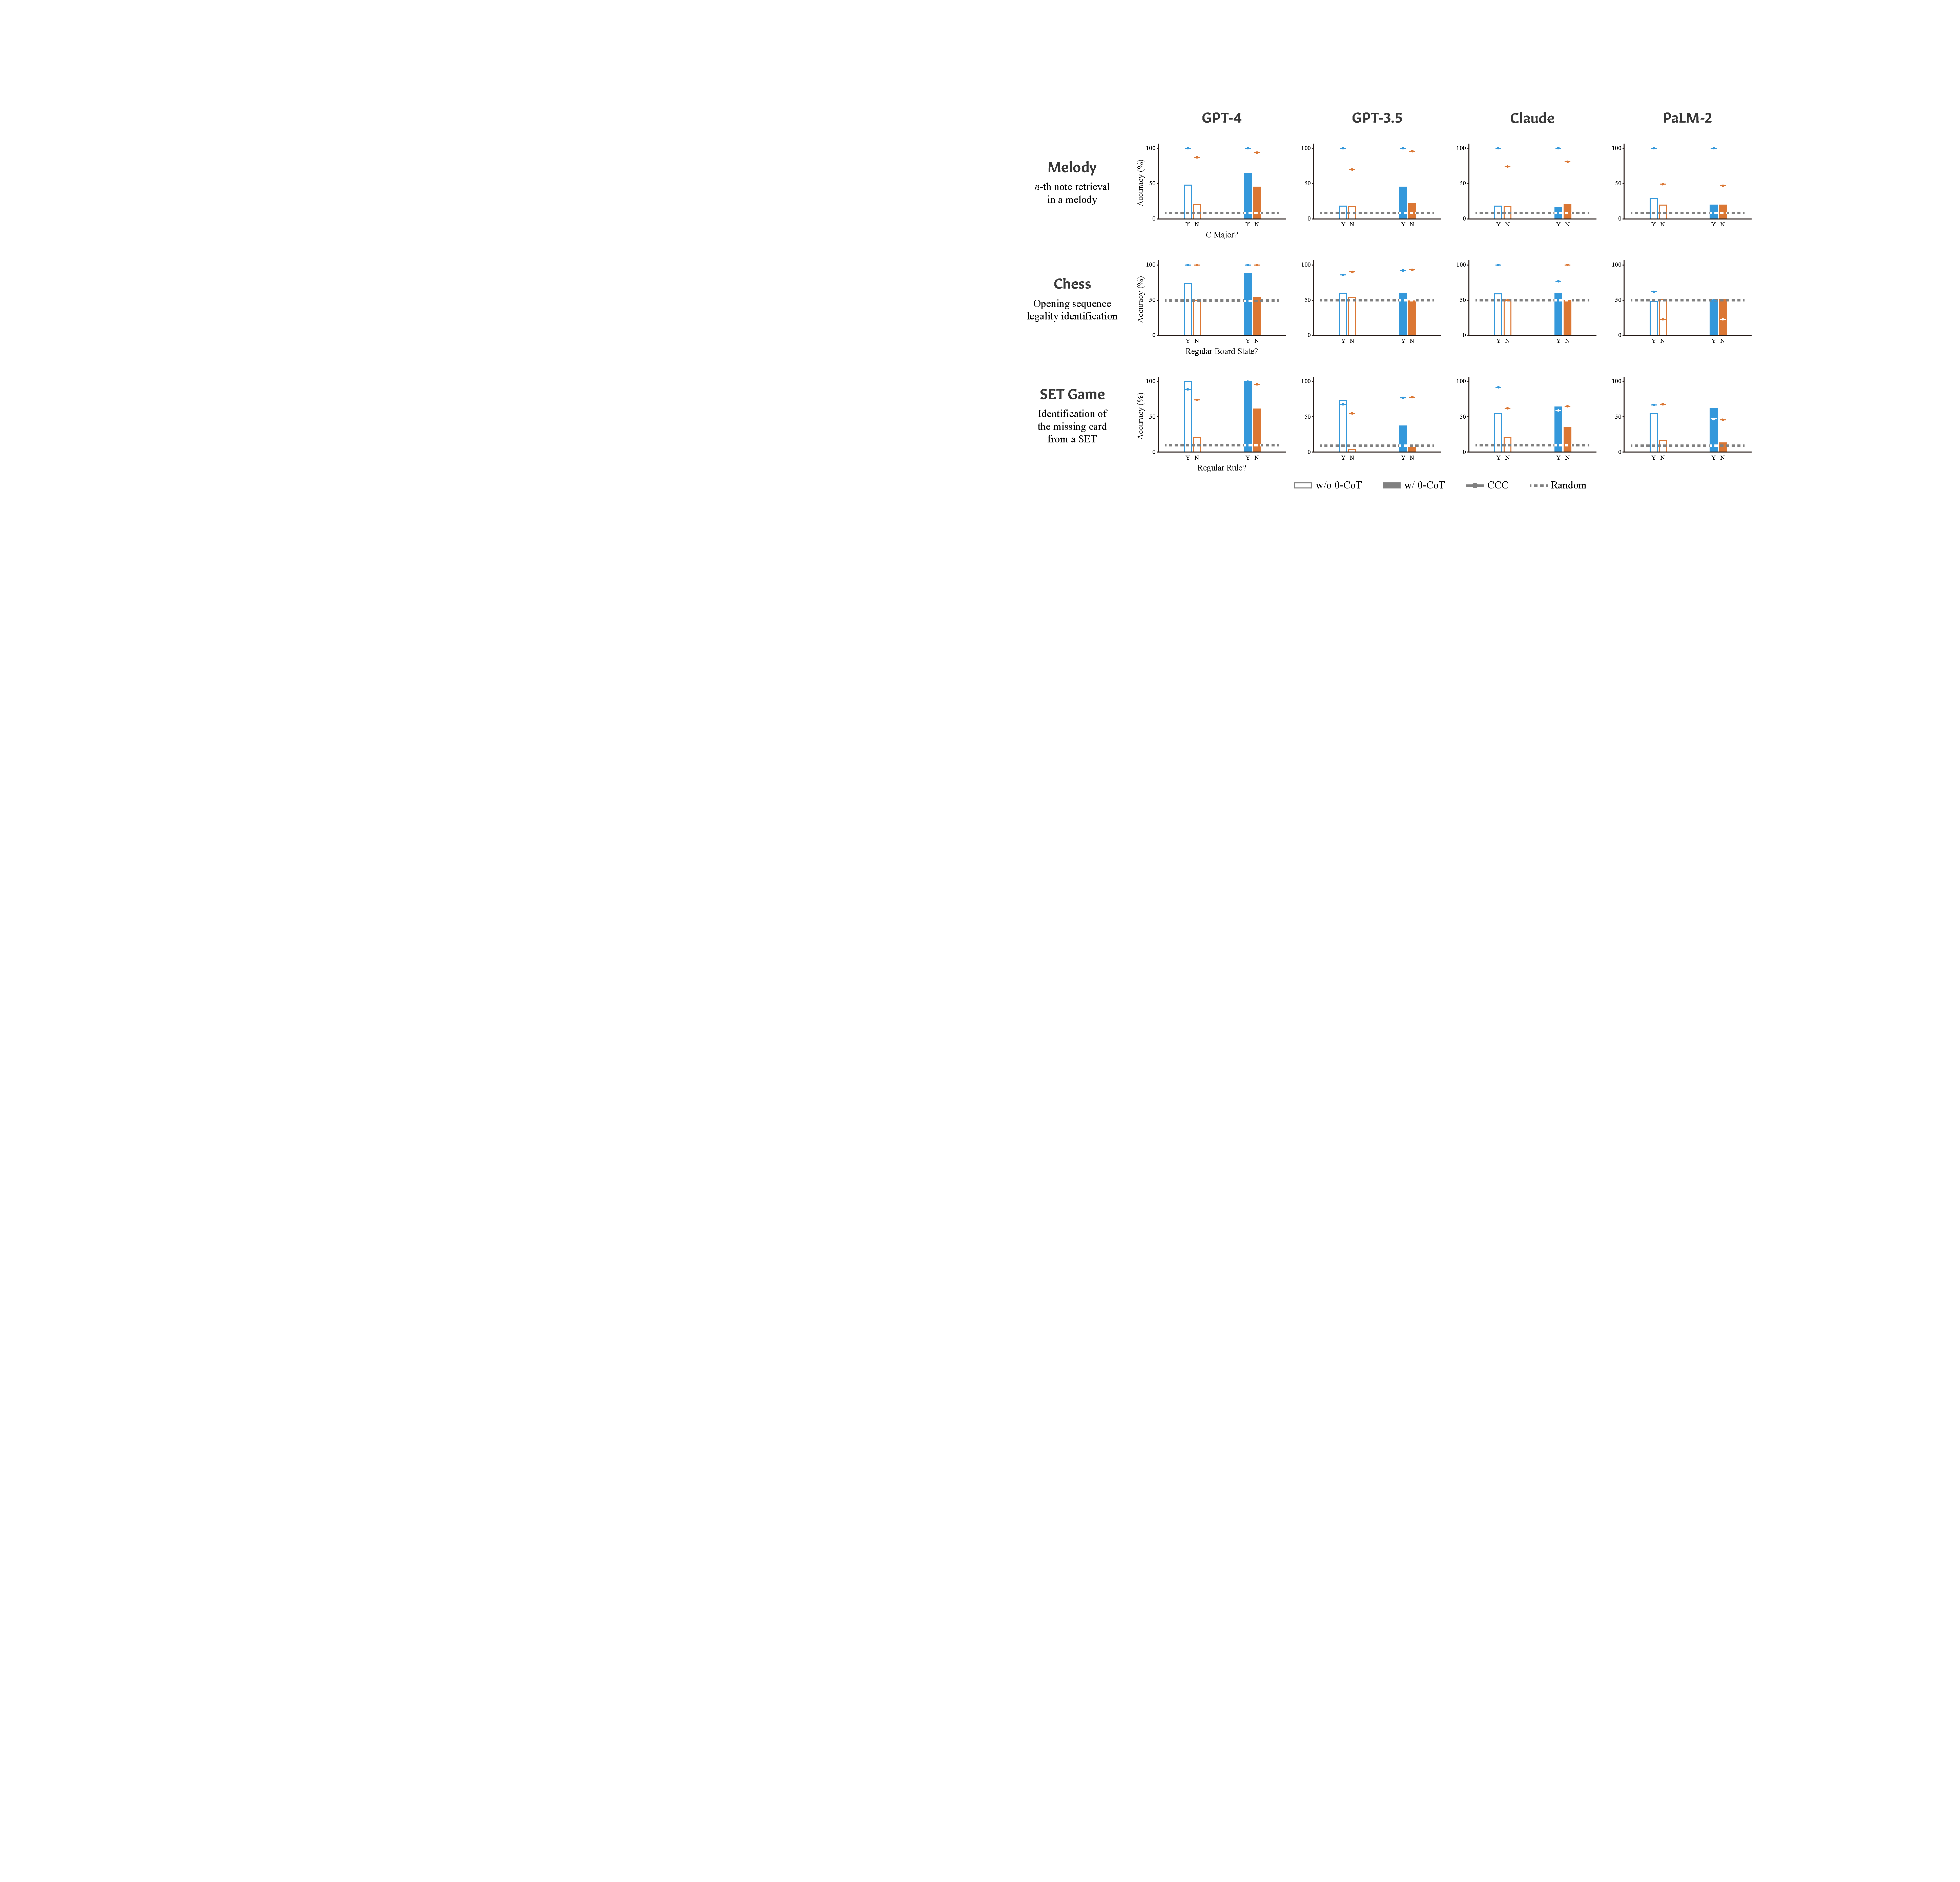
\includegraphics[width=\textwidth]{figures/results-2.pdf}
    \caption{
    Main results (continued).
    The \textcolor{real}{blue} and \textcolor{cf}{orange} bars represent the \textcolor{real}{default} and \textcolor{cf}{counterfactual} conditions respectively, either  with or without 0-shot chain-of-thought (0-CoT). CCC is the counterfactual comprehension check (\S\ref{subsec:ccc}), but when applicable, we report it for the default setting too.
    Random performance is marked whenever nontrivial.
    PaLM-2 here is not the largest version (\S\ref{sec:results}).
    Counterfactual performance is consistently lower than the default task performance, while CCC is usually high.
    \S\ref{sec:raw-results} reports numeric results.}
    \label{fig:results-2}
\end{figure*}

\vspace{-1mm}
\section{Results} \label{sec:results}
\vspace{-1mm}
For each task, we evaluate GPT-4 (\texttt{gpt-4-0314}; \citealp{gpt4}), GPT-3.5 (\texttt{gpt-3.5-turbo-0301}), Claude (\texttt{claude-v1.3}; \citealp{claude}), and PaLM-2 (\texttt{text-bison-001}; \citealp{palm2}). As these are closed-source models, we do not have any information regarding their size, architecture, and pretaining details.\footnote{We also explored open-source models in preliminary experiments, but found that they possess unsatisfactory instruction-following ability, to the point that often their output cannot be meaningfully parsed into a prediction. We therefore do not include these models.} We note that the largest PaLM-2 model is not publicly accessible, and we can only test the second-largest version.
For each task, we experiment both with and without encouraging the model to reason step by step, by adding the phrase ``\texttt{Let's think step by step.}'' in our prompts~\citep{kojima2023large,Reynolds2021prompt}. Following \citet{kojima2023large}, we refer to this step-by-step setup as zero-shot chain-of-thought prompting (\textbf{0-CoT}; \citealp{nye2021work,wei2022chain}).
We include all  prompts in \S\ref{sec:prompts}.

Figures~\ref{fig:results-1} and \ref{fig:results-2} show our results. 
\S\ref{sec:raw-results} contains the numeric version.
We see a consistent pattern where LMs perform substantially worse on the counterfactual task variants, both with and without 0-shot CoT. For most cases, LMs exhibit an above-random counterfactual performance, suggesting some degree of the targeted ability. However, when the CCC accuracy is high, as is usually the case for GPT-4 and in select settings for other models too, the gaps in default vs. counterfactual task performance demonstrate limitations in their abstract capacity to solve the target task.
When the CCC accuracy is lower, the failure of counterfactual world comprehension would be a confounder to this conclusion, but often the gaps are so large (sometimes even dropping from near-perfect to near-zero, such as for arithmetic) that they are nonetheless strongly indicative of non-transferable, default-condition-specific implementations of the original task. The fact that the LMs sometimes cannot evaluate the CCC well under the counterfactual conditions, but can do so under the default conditions (e.g., for arithmetic, programming, drawing, etc.) itself also points to overfitting to the latter.
